\section{Fibonacci sequence}
\subsection{Aim}
To generate first n Fibonacci numbers.

\subsection{Code}
\begin{lstlisting}
ORG 0000H

MOV R0, #08H
MOV DPTR, #100H

MOV A, #00H
MOVX @DPTR, A
INC DPTR
MOV A, #01H
MOVX @DPTR, A

LOOP:
	MOV A, DPL
	SUBB A, #1
	MOV DPL, A
	MOV A, DPH
	SUBB A, #0H
	MOV DPH, A

	MOVX A, @DPTR
	INC DPTR
	MOV R1, A
	MOVX A, @DPTR
	INC DPTR
	ADD A, R1
	MOVX @DPTR, A

	DJNZ R0, LOOP
END
\end{lstlisting}

\subsection{Output}
\textbf{Input} 08H (R0)\\
\textbf{Output} 00H, 01H, 01H, 02H, 03H, 05H, 08H, 0DH, 15H, 22H (At locations from \#100H of XDATA)\\
\begin{center}
	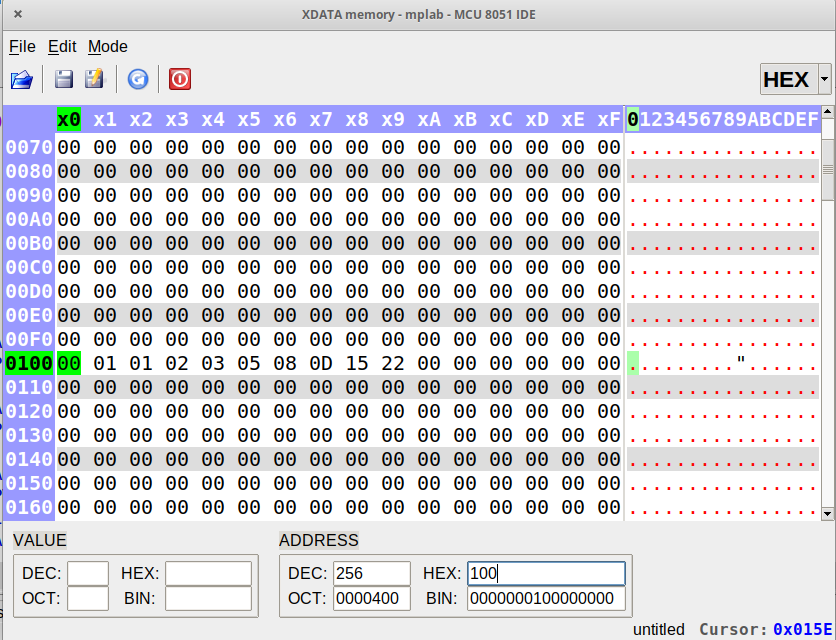
\includegraphics[width=\textwidth]{img/p28.png}
\end{center}


\subsection{Result}
First n Fibonacci sequence was generated in mcu8051ide